%-----------------------------------------------------------------------------%
\chapter{\topikSatu}
%-----------------------------------------------------------------------------%

%-----------------------------------------------------------------------------%
\section{Pendahuluan}
%-----------------------------------------------------------------------------%
Topik eksperimen pertama adalah perkalian matriks-vektor dan perkalian matriks bujur sangkar dengan beberbagai algoritma paralel. 

\subsection{Perkalian Matriks-Vektor} 

\subsubsection{Row-Wise Decomposition}

Algoritma paralel perkalian matriks-vektor yang paling sederhana, yaitu memecah proses perkalian berdasarkan baris matriks (\f{row-wise}). Setiap prosesor akan bertanggung jawab untuk mengalikan sebuah baris matriks dan vektor pada satu waktu. Jika jumlah prosesor ($np$) lebih sedikit dari jumlah baris matriks ($r$) maka setiap prosesor bertugas mengalikan $n = \frac{r}{np}$ secara sekuensial.

\begin{figure}
	\centering
	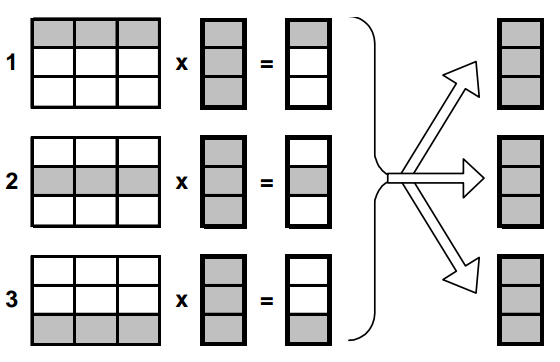
\includegraphics[width=0.75\textwidth]
	{pics/mv_rowwise}
	\caption{Perkalian matriks-vektor Row-Wise Decomposition}
	\label{fig:mv_rowwise}
\end{figure}  

\subsubsection{Column-wise Decomposition}

Algoritma perkalian matriks-vektor ini merupakan alternatif dari \f{row-wise decomposition} di mana pemecahan proses perkalian dilakukan berdasarkan kolom matriks. Setiap proses akan mengalikan sebuah kolom matriks dan sebuah elemen vektor pada satu waktu. Mirip dengan algoritma \f{row-wise decomposition}, jika jumlah prosesor ($np$) lebih sedikit dari jumlah kolom matriks ($c$) maka setiap prosesor bertugas mengalikan $n = \frac{c}{np}$ secara sekuensial.

\begin{figure}
	\centering
	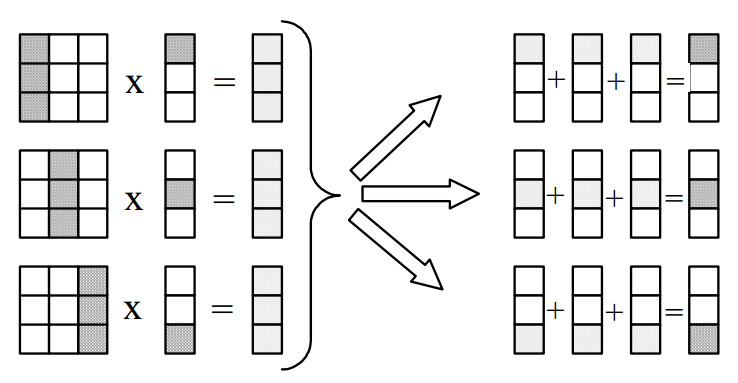
\includegraphics[width=0.9\textwidth]
	{pics/mv_colwise}
	\caption{Perkalian matriks-vektor Column-Wise Decomposition}
	\label{fig:mv_colwise}
\end{figure}  

\subsection{Checkerboard Decomposition}

%-----------------------------------------------------------------------------%
\section{Eksperimen}
%-----------------------------------------------------------------------------%
Pada bagian ini akan dijelaskan mengenai definisi permasalahan 
yang \saya~hadapi dan ingin diselesaikan serta asumsi dan batasan 
yang digunakan dalam menyelesaikannya.


%-----------------------------------------------------------------------------%
\section{Analisis \& Kesimpulan}
%-----------------------------------------------------------------------------%




